\documentclass[10pt,letterpaper,twoside]{article}
\usepackage{code/manuscript_assets/researchpreprint}
\usepackage{amsmath,amssymb,mathtools,amsthm,booktabs,graphicx}
\usepackage[hidelinks]{hyperref}
\newcommand{\norm}[1]{\left\lVert#1\right\rVert}
\newtheorem{theorem}{Theorem}
\begin{document}
\title{Safety-Gated Spectral Reconstruction of Experimental Ramsey Fringes}
\author{Molena Huynh}\email{molena.huynh@jmp.com}
\affiliation{North Carolina State University}
\maketitle

\begin{abstract}
A single reconstruction rule is often poorly matched to a heterogeneous
collection of experimental fringes. A trace-local procedure is introduced
that retains linear interpolation unless nested development points support a
regularized spectral model by a fixed safety margin. Each spectral candidate
uses 4, 6, 8, or 10 harmonics and a Bohr-anchored Sobolev penalty; independent
trace blocks are solved without materializing the global block-diagonal
design. A deterministic selection theorem bounds the selected test loss in
terms of the best candidate whenever development and test losses are uniformly
close. A second theorem proves exact equivalence of block and explicit normal
equations and reduces design storage from $O(NTp)$ to $O(Np)$. Evaluation uses
40,787 measured probabilities from 177 trapped-ion Ramsey fringes in an
authenticated CC-BY archive. Every fourth phase point is held out; disjoint
outer-training points select among 29 candidates per trace. The fixed
five-percent gate lowers mean held-out RMSE from 0.09434 to 0.09146 and pooled
RMSE from 0.09947 to 0.09732. Improvement occurs in every state-group mean and
69 individual traces; unfavorable accepted-model cases are retained. At 32
traces, the equivalent block solve is 17.1 times faster in the recorded CPU
experiment and stores 1.03 MB rather than 31.55 MB. These results establish a
guarded reconstruction and representation improvement on the stated archive,
not universal spectral superiority or dynamical-system identification.
\end{abstract}

\section{Measured-fringe setting}

The record contains $N=40{,}787$ excitation probabilities from $T=177$
Ramsey fringes spanning eight prepared-state labels
~\cite{kovalenko2025ramsey}. Numeric worksheet cells are transcribed without
loss to a checksum-locked CSV. The complete archive and derived-file SHA-256
digests are stored in the released result record. Every reported result is
regenerated from that file.

For trace $t$, measurements $(\phi_{ti},y_{ti})$ are divided by phase index.
Indices congruent to zero modulo four form the outer test set. Among the
remaining points, indices congruent to three modulo eight form an inner
development set; all other points form the inner fit set. Thus no outer-test
probability participates in candidate construction or selection.

Piecewise-linear interpolation is a strong local comparator for these densely
sampled fringes. A global ten-harmonic fit improves the cleanest state group
but degrades the heterogeneous collection. The proposed rule treats linear
interpolation as a protected default and permits a spectral replacement only
when its inner-development improvement exceeds a predeclared margin.

\section{Safety-gated block spectral fit}

For a candidate harmonic count $h$, define
\begin{equation}
 \begin{aligned}
 f_h(\phi)&=[1,\sin\phi,\cos\phi,\ldots,\\
 &\hspace{2.2cm}\sin(h\phi),\cos(h\phi)]\in\mathbb R^p,\\
 p&=2h+1.
 \end{aligned}
\end{equation}
Let $F_t$ contain inner-fit rows and $y_t$ the corresponding probabilities.
Candidate coefficients solve
\begin{equation}
 \widehat\theta_t(h,\lambda)=
 \arg\min_\theta \norm{F_t\theta-y_t}_2^2+
 \theta^T(10^{-2}I+\lambda D_h)\theta, \label{eq:local}
\end{equation}
where the intercept and fourth harmonic have zero entries in $D_h$, while
the sine and cosine entries for harmonic $k\ne4$ equal $k^2$. The grid is
$h\in\{4,6,8,10\}$ and
$\lambda\in\{0,0.03,0.1,0.3,1,3,10\}$.

Let $\widehat L_0$ be linear-interpolation RMSE on inner development points
and $\widehat L_s$ the minimum spectral-development RMSE. With $\tau=0.05$,
the spectral minimizer is accepted only if
\begin{equation}
 \widehat L_s<(1-\tau)\widehat L_0. \label{eq:gate}
\end{equation}
The accepted model is refitted on all outer-training points. Otherwise linear
interpolation is retained. This gives 29 candidates, including the protected
default, for every trace.

\begin{theorem}[Conditional selection bound]
\label{thm:gate}
Let $\mathcal C$ contain the default and all spectral candidates. Suppose
development and test losses obey $|\widehat L_c-L_c|\le\epsilon$ for every
$c\in\mathcal C$. The rule in Eq.~\eqref{eq:gate} returns $\widehat c$ with
\begin{equation}
 L_{\widehat c}\le
 \frac{\min_{c\in\mathcal C}L_c+\epsilon}{1-\tau}+\epsilon. \label{eq:risk}
\end{equation}
\end{theorem}
\begin{proof}
If the spectral candidate is accepted, it is the global development minimizer.
If the default is retained, the best spectral loss is at least
$(1-\tau)\widehat L_0$, hence
$\widehat L_0\le\min_c\widehat L_c/(1-\tau)$. Both cases give
$\widehat L_{\widehat c}\le\min_c\widehat L_c/(1-\tau)$.
Applying the assumed discrepancy to the selected candidate and to the
test-loss minimizer proves Eq.~\eqref{eq:risk}.
\end{proof}

The theorem is deterministic and conditional. It exposes the role of the
safety margin without asserting that one inner slice estimates future loss
uniformly. The trace-level confirmation panel reports observed failures of
that premise.

\section{Matrix-free block elimination}

Let $F=\operatorname{diag}(F_1,\ldots,F_T)$ and
$R=\operatorname{diag}(R_1,\ldots,R_T)$ denote the explicit global design and
regularizer. The implementation stores local feature rows and trace indices,
applying $F$ and $F^T$ by indexed reductions.

\begin{theorem}[Exact block equivalence and cost]
\label{thm:block}
If every $F_t^TF_t+R_t$ is positive definite, the explicit solution equals
the concatenation of
\begin{equation}
 \widehat\theta_t=(F_t^TF_t+R_t)^{-1}F_t^Ty_t.
\end{equation}
For at most $p$ local features and $N$ total fit rows, block elimination costs
$O(Np^2+Tp^3)$ arithmetic and $O(Np+Tp^2)$ storage. Explicit global design
storage is $O(NTp)$.
\end{theorem}
\begin{proof}
The normal matrix is
\begin{equation}
 F^TF+R=\operatorname{diag}(F_1^TF_1+R_1,\ldots,F_T^TF_T+R_T).
\end{equation}
Its inverse contains the local inverses, proving equality. Accumulating local
Gram matrices costs $O(Np^2)$, their factorizations cost $O(Tp^3)$, and local
features plus Gram matrices require $O(Np+Tp^2)$ storage. An explicit row has
$Tp$ columns, giving $O(NTp)$ storage.
\end{proof}

\section{Experimental results}

The gate accepts a spectral model for 91 of 177 traces. Table~\ref{tab:states}
shows that mean held-out RMSE decreases in every state group. Across all
traces, mean RMSE falls by 3.04 percent and pooled squared error falls by 4.28
percent.

\begin{table}[t]
\caption{Outer-test RMSE by prepared-state label. Values are means over traces;
the last column records accepted spectral models.}
\label{tab:states}
\begin{ruledtabular}\begin{tabular}{lrrrr}
State & Traces & Gated & Linear & Selected\\ \hline
$0+1$ & 11 & .04733 & .05484 & 9\\
$0+2$ & 10 & .04780 & .05191 & 5\\
$0+3$ & 48 & .10693 & .10772 & 15\\
$0+4$ & 41 & .11246 & .11454 & 18\\
$0+6$ & 24 & .12774 & .13086 & 16\\
$1+2$ & 15 & .05646 & .05984 & 8\\
$1+3$ & 12 & .06156 & .06436 & 8\\
$2+3$ & 16 & .04973 & .05613 & 12\\ \hline
All & 177 & .09146 & .09434 & 91
\end{tabular}\end{ruledtabular}
\end{table}

Figure~\ref{fig:evidence}(a) displays the state-stratified comparison. Panel
(b) retains every trace rather than only a favorable subset. The gate improves
69 traces, ties 86 traces that retain interpolation, and loses on 22 accepted
spectral traces. Panel (c) relates the inner selection statistic to outer-test
gain; points below zero are explicit selection failures.

\begin{figure}[t]
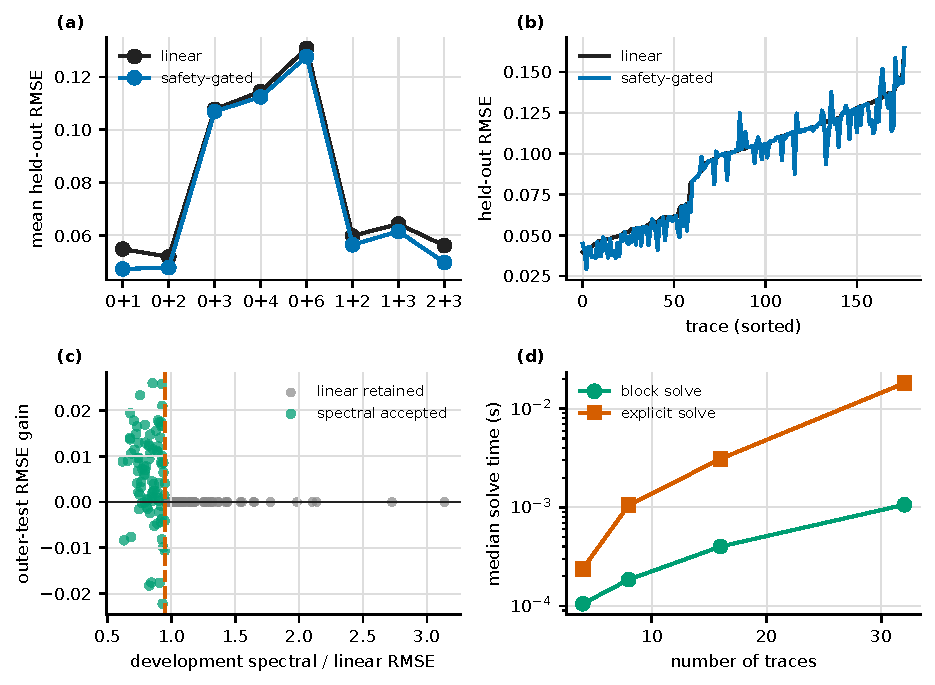
\includegraphics[width=\textwidth]{code/manuscript_assets/figures/adaptive/adaptive_ramsey.pdf}
\caption{Accuracy, selection, and cost evidence. (a) Mean outer-test RMSE by
state group. (b) Every trace, sorted by interpolation RMSE. (c) Inner
spectral-to-linear error ratio against outer-test gain; the dashed line is the
fixed gate. (d) Equivalent explicit and block-solve CPU time.}
\label{fig:evidence}
\end{figure}

The representation comparison in Table~\ref{tab:compute} solves identical
normal equations and verifies predictions to $9.44\times10^{-16}$ at 32
traces. The full 177-trace fit stores 5.37 MB in local features and indices;
the corresponding explicit design would occupy 0.907 GB. These numbers refer
to representation and solve cost, while nested selection performs additional
small local solves.

\begin{table}[b]
\caption{Measured equivalent-solve scaling. Times are medians of three CPU
runs; memory is stored design representation.}
\label{tab:compute}
\begin{ruledtabular}\begin{tabular}{rrrrr}
Traces & Block (ms) & Explicit (ms) & Speedup & MB ratio\\ \hline
4 & 0.105 & 0.238 & 2.3 & 3.8\\
8 & 0.185 & 1.052 & 5.7 & 7.6\\
16 & 0.401 & 3.108 & 7.8 & 15.3\\
32 & 1.062 & 18.181 & 17.1 & 30.5
\end{tabular}\end{ruledtabular}
\end{table}

\section{Scope}

The archive supplies broad within-experiment heterogeneity but not independent
devices or acquisition campaigns. The five-percent gate is fixed before the
outer evaluation, yet the conditional discrepancy in
Theorem~\ref{thm:gate} is not certified from one inner slice. The 22
accepted-model losses remain essential evidence. Spectral coefficients
describe measured phase fringes and do not identify a Hamiltonian or
open-system generator. The supported conclusion is computational and
predictive: guarded local selection improves aggregate held-out reconstruction
on this archive while preserving an interpolation fallback and an exact
block-elimination implementation.

\bibliographystyle{plainnat}
\bibliography{code/manuscript_assets/references}
\end{document}
